\section{Jakub Liana}
\label{sec:Linas}

\subsection{Wyrazenie matematyczne}
    Kazdy uwielbia twierdzenia Eulera, wiec: \[e^{\pi i}=-1\]
\subsection{Zdjecie}
    Teraz czas na cos ciekawszego, prosze spojrzec na zdjecie \ref{fig:s13}
    \begin{figure}[h]
        \centering
        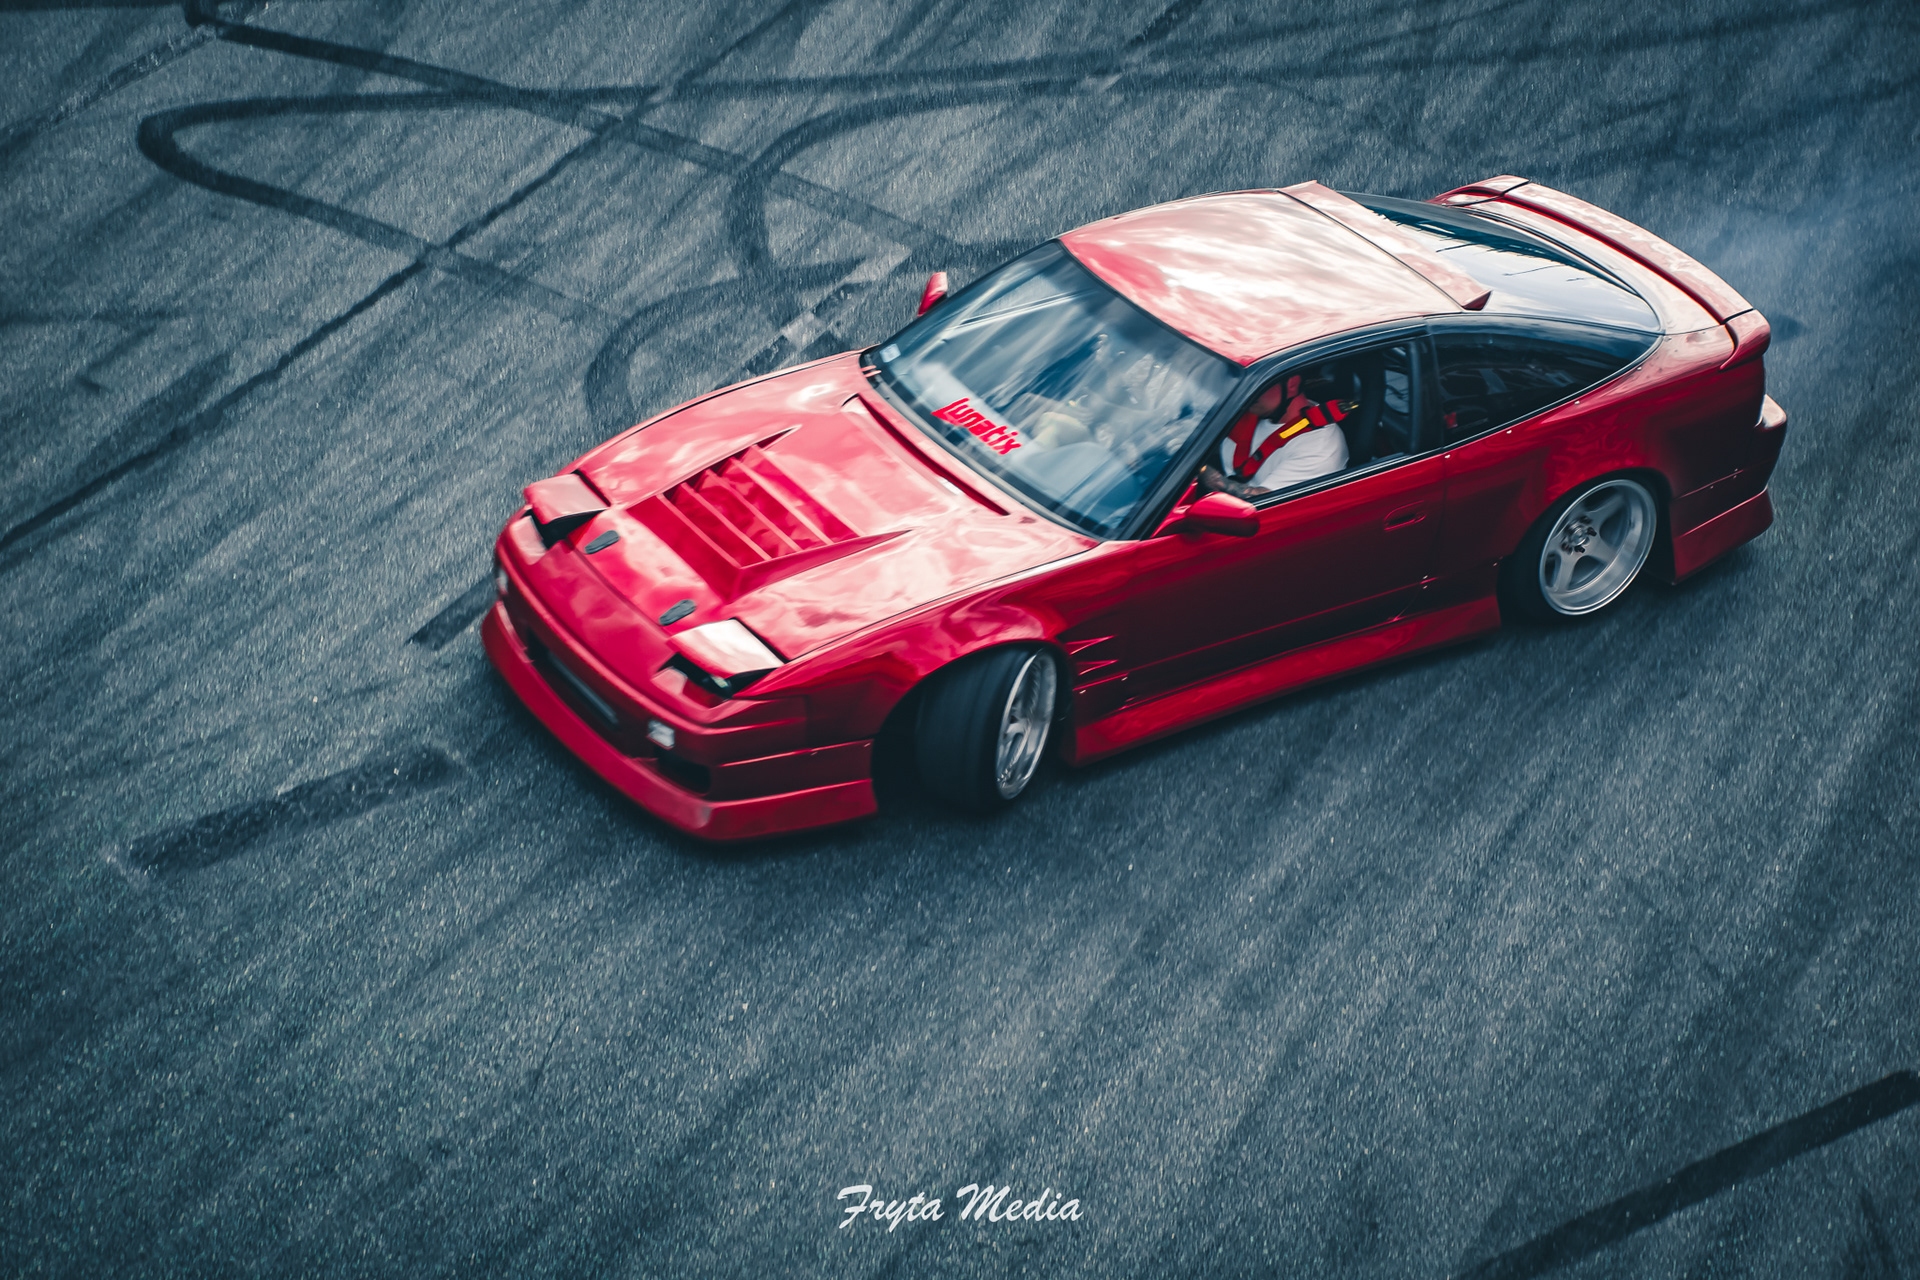
\includegraphics[width=1\textwidth]{pictures/s13.jpg}
        \caption{Piekne autka tylko u mnie}
        \label{fig:s13}
    \end{figure}
    \newpage
\subsection{Tabela}
    Przykladowa wygenerowana tabela
    \begin{table}[htbp]
\label{lab:tabela}
        \begin{tabular}{llrll}
            \cline{1-3}
            \multicolumn{1}{|l|}{\textit{1}} & \multicolumn{1}{l|}{{\ul 2}} & \multicolumn{1}{r|}{\textbf{626}} &  &  \\ \cline{1-3}
            \multicolumn{1}{|l|}{\textit{1}} & \multicolumn{1}{l|}{{\ul 2}} & \multicolumn{1}{r|}{\textbf{323}} &  &  \\ \cline{1-3}
            \multicolumn{1}{|c|}{mazda}      & \multicolumn{1}{c|}{nissan}  & \multicolumn{1}{c|}{toyota}       &  &  \\ \cline{1-3}
                                             &                              & \multicolumn{1}{l}{}              &  & 
        \end{tabular}
    \end{table}
    \\Warto zauwazyc, ze w 3 rzedzie tabeli \ref{lab:tabela} nie ma napisow, natomiast ten tekst jest tylko po to, by wykorzystac \verb|\ref{}|
\subsection{Listy}
    \subsubsection{Lista numerowana}
        \begin{enumerate}
            \item Pierwszy numerowany element
            \item Drugi numerowany element
            \begin{enumerate}
                \item zagniezdzony element
            \end{enumerate}
        \end{enumerate}
    \subsubsection{Lista nienumerowana}
        \begin{itemize}
            \item Pierwszy element
            \item Drugi element
            \begin{itemize}
                \item zagniezdzony element
            \end{itemize}
        \end{itemize}
\subsection{Krotki tekst}
    To jest pierwszy akapit, jest on \textbf{pogrubiony} oraz \textit{pochylony} \\
    \underline{Natomiast w drugim akapicie wszystko jest podkreslone}